

    \item Two independent harmonic oscillators of equal mass are oscillating about the origin with angular frequencies \( \omega_1 \) and \( \omega_2 \) and have total energies \( E_1 \) and \( E_2 \), respectively. The variations of their momenta \( p \) with positions \( x \) are shown in the figures. If \( \frac{a}{R} = n \), then the correct equation(s) is(are)
    \begin{center}
        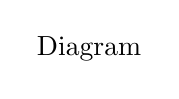
\begin{tikzpicture}
        \node {Diagram};
        \end{tikzpicture}
        \end{center}
        \begin{tasks}(2)
            \task \( E_1\omega_1 = E_2\omega_2 \)
            \task \( \frac{\omega_2}{\omega_1} = n^2 \)
            \task \( \omega_1\omega_2 = n^2 \)
            \task \( \frac{E_1}{\omega_1} = \frac{E_2}{\omega_2} \)
        \end{tasks}



